\chapter{Applications d'algorithmes en IA}

\section{Introduction}
L'intelligence artificielle repose sur des algorithmes sophistiqués pour prendre des décisions, analyser des données et résoudre des problèmes complexes. Ce chapitre explore les algorithmes populaires de l'IA en mettant l’accent sur leur fonctionnement étape par étape et sur des exemples concrets qui illustrent leur application.

\section{Algorithmes d'Apprentissage Supervisé}

\subsection{Régression Linéaire}
La \textbf{régression linéaire} est utilisée pour prédire une valeur numérique continue (comme un prix ou une température) en fonction d'une ou plusieurs variables.

\begin{itemize}
	\item \textbf{Idée de base} : Imaginez un nuage de points sur un graphique où l'axe $x$ représente une variable (par exemple, la taille d’une maison) et l'axe $y$ représente le résultat (comme le prix de la maison). La régression linéaire cherche à tracer une ligne qui passe le plus près possible de ces points.
	\item \textbf{Étapes de l’algorithme} :
	\begin{enumerate}
		\item \textbf{Préparer les données} : Regroupez les données en paires $(x, y)$.
		\item \textbf{Déterminer l’équation} : Une ligne est définie par $y = ax + b$.
		\item \textbf{Ajuster la ligne} : Trouvez $a$ et $b$ pour minimiser l’erreur.
		\item \textbf{Prédire} : Utilisez $y = ax + b$ pour de nouvelles valeurs de $x$.
	\end{enumerate}
\end{itemize}

\begin{table}[h]
	\centering
	\caption{Données pour la régression linéaire}
	\begin{tabular}{|c|c|}
		\hline
		Surface (m²) & Prix (MGA) \\ \hline
		50           & 70,000,000 \\ \hline
		75           & 95,000,000 \\ \hline
		100          & 130,000,000 \\ \hline
	\end{tabular}
\end{table}

\begin{figure}[h]
	\centering
	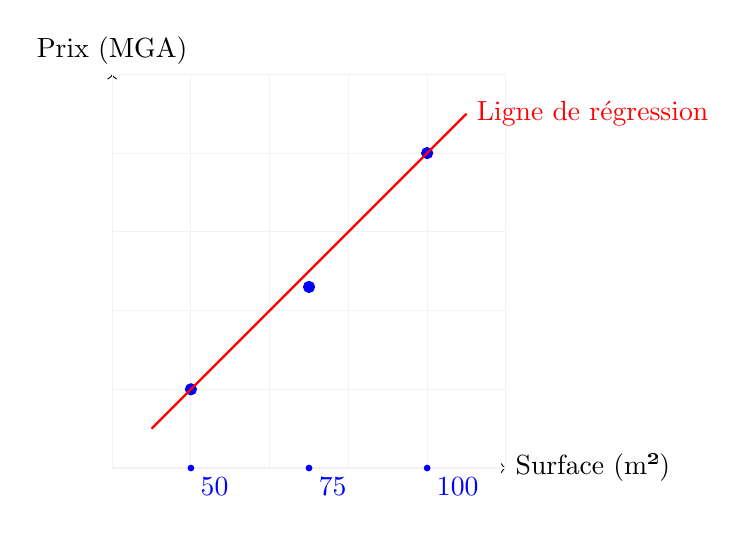
\begin{tikzpicture}
		% Axes
		\draw[->] (0,0) -- (5,0) node[right] {Surface (m²)};
		\draw[->] (0,0) -- (0,5) node[above] {Prix (MGA)};
		
		% Gridlines
		\draw[gray!10, thin] (0,0) grid (5,5);
		
		% Points
		\filldraw[blue] (1,1) circle (2pt) node[below left] {};
		\filldraw[blue] (2.5,2.3) circle (2pt) node[below right] {};
		\filldraw[blue] (4,4) circle (2pt) node[below right] {};
		\filldraw[blue] (1,0) circle (1pt) node[below right] {50};
		\filldraw[blue] (2.5,0) circle (1pt) node[below right] {75};
		\filldraw[blue] (4,0) circle (1pt) node[below right] {100};
		
		% Regression line
		\draw[red, thick] (0.5,0.5) -- (4.5,4.5) node[right] {Ligne de régression};
	\end{tikzpicture}
	\caption{Régression linéaire sur des données simulées.}
\end{figure}

\section*{Exercice : Implémenter la Régression Linéaire}
\begin{enumerate}
	\item  Écrivez un programme en C qui :  
\begin{itemize}
	\item Accepte les paires $(x, y)$ en entrée.  
	\item Calcule les coefficients $a$ et $b$.  
	\item Prédit $y$ pour une nouvelle valeur $x$.  
\end{itemize}
\item  Utilisez les données du tableau ci-dessus et prédisez $y$ pour $x = 80$.  
\end{enumerate}

\subsection{Régression Logistique}
La \textbf{régression logistique} est utilisée pour prédire une probabilité binaire, comme "oui/non" ou "succès/échec".

\begin{itemize}
	\item \textbf{Idée de base} : Contrairement à la régression linéaire, la régression logistique utilise une \textit{fonction sigmoïde} pour transformer un score $z$ en une probabilité :
	\[
	P = \frac{1}{1 + e^{-z}}
	\]
	\item \textbf{Étapes de l’algorithme} :
	\begin{enumerate}
		\item Calculez $z$ avec $z = a \cdot x + b$.
		\item Appliquez la fonction sigmoïde pour obtenir $P$.
		\item Comparez $P$ avec un seuil (e.g., 0,5) pour décider "oui" ou "non".
	\end{enumerate}
\end{itemize}

\begin{table}[h]
	\centering
	\caption{Exemple pour la régression logistique}
	\begin{tabular}{|c|c|c|}
		\hline
		Temps (minutes) & Pages visitées & $z$ \\ \hline
		12              & 7              & $z = 2.3$ \\ \hline
	\end{tabular}
\end{table}

\begin{figure}[h]
	\centering
	\begin{tikzpicture}
		% Axes
		\draw[->] (-5,0) -- (5,0) node[right] {Score $z$};
		\draw[->] (0,0) -- (0,5) node[above] {Probabilité $P$};
		\draw[dashed] (-5, 4) -- (5,4) node[right] { $P=1$};
		% Sigmoid curve
		\draw[blue, thick, smooth, domain=-5:5, samples=100] plot (\x,{4/(1 + exp(-\x))});
		
		% Threshold line
		\draw[dashed] (-5,2) -- (5,2) node[right] {Seuil $P = 0.5$};
	\end{tikzpicture}
	\caption{Courbe sigmoïde pour la régression logistique.}
\end{figure}

\section*{Exercice : Implémenter la Régression Logistique}
\begin{enumerate}
	\item  Écrivez un programme en C qui :  
\begin{itemize}
	\item Calcule $z$ pour une valeur donnée.  
	\item Transforme $z$ en $P$ à l’aide de la fonction sigmoïde.  
	\item Compare $P$ avec un seuil pour afficher "Oui" ou "Non".  
\end{itemize}
\item Utilisez les données du tableau ci-dessus et prédisez si le client achètera.
\end{enumerate}

\subsection{Clustering avec K-means}
L’algorithme \textbf{K-means} regroupe des données en plusieurs groupes appelés \textit{clusters}.

\begin{itemize}
	\item \textbf{Idée de base} : Divisez les données en $K$ groupes, chaque groupe ayant un centre (\textit{centroïde}).
	\item \textbf{Étapes de l’algorithme} :
	\begin{enumerate}
		\item Choisissez $K$ centroïdes aléatoires.
		\item Assignez chaque point au centroïde le plus proche.
		\item Recalculez les centroïdes en prenant la moyenne des points.
		\item Répétez jusqu'à ce que les centroïdes ne changent plus.
	\end{enumerate}
\end{itemize}

\begin{table}[h]
	\centering
	\caption{Données pour K-means}
	\begin{tabular}{|c|c|}
		\hline
		Point & Coordonnées $(x, y)$ \\ \hline
		A     & (1, 2)              \\ \hline
		B     & (3, 4)              \\ \hline
		C     & (5, 6)              \\ \hline
		D     & (8, 9)              \\ \hline
	\end{tabular}
\end{table}

\begin{figure}[h]
	\centering
	\begin{tikzpicture}
		% Axes
		\draw[->] (0,0) -- (6,0) node[right] {Caractéristique 1};
		\draw[->] (0,0) -- (0,6) node[above] {Caractéristique 2};
		
		% Points
		\filldraw[red] (1,1) circle (2pt) node[below left] {A};
		\filldraw[red] (1.5,1.5) circle (2pt) node[below right] {B};
		\filldraw[blue] (4,4) circle (2pt) node[below] {C};
		\filldraw[blue] (4.5,4.5) circle (2pt) node[above right] {D};
		
		% Centroids
		\filldraw[black] (1.25,1.25) circle (3pt) node[above left] {C1};
		\filldraw[black] (4.25,4.25) circle (3pt) node[below right] {C2};
	\end{tikzpicture}
	\caption{Clustering K-means avec deux clusters.}
\end{figure}

\section*{Exercice : Implémenter K-means}
\begin{enumerate}
	\item  Écrivez un programme en C qui :  
\begin{itemize}
	\item Accepte une liste de points $(x, y)$.  
	\item Initialise 2 centroïdes aléatoires.  
	\item Assigne chaque point au centroïde le plus proche.  
	\item Recalcule les centroïdes et affiche les groupes finaux.  
\end{itemize}
\item  Utilisez les données du tableau ci-dessus. 
\end{enumerate}
